\chapter*{Descrizione Progetto}
\renewcommand{\thesection}{\arabic{section}}
Lo scopo di questo progetto consiste nella valutazione dei costi operativi di un call center con operatività 24 ore su 24, 7 giorni su 7 per conto di un'azienda del settore utilities.
Nel nostro caso è stato scelto di analizzare le stime degli \ac{OPEX} riguardanti i primi mesi a partire dell'apertura del call center nell'anno solare 2016.
\section[Organigramma Aziendale]{Organigramma Aziendale}


\begin{tikzpicture}[
  level 1/.style={sibling distance=55mm},
  edge from parent/.style={->,draw},
  >=latex]

% root of the the initial tree, level 1
\node[root] {CEO}
% The first level, as children of the initial tree
  child {node[level 2] (c1) {Manager \#1}}
  child {node[level 2] (c2) {Manager \#2}}
  child {node[level 2] (c3) {Manager \#3}};

% The second level, relatively positioned nodes
\begin{scope}[every node/.style={level 3}]
\node [below of = c1, xshift=30pt] (c11) {Centralinista \#1};
\node [below of = c11] (c12) {Centralinista ...};
\node [below of = c12] (c13) {Centralinista \#5};

\node [below of = c2, xshift=30pt] (c21) {Centralinista \#6};
\node [below of = c21] (c22) {Centralinista ...};
\node [below of = c22] (c23) {Centralinista \#10};

\node [below of = c3, xshift=30pt] (c31) {Centralinista \#11};
\node [below of = c31] (c32) {Centralinista ...};
\node [below of = c32] (c33) {Centralinista \#15};
\end{scope}

% lines from each level 1 node to every one of its "children"
\foreach \value in {1,2,3}
  \draw[->] (c1.195) |- (c1\value.west);

\foreach \value in {1,...,3}
  \draw[->] (c2.195) |- (c2\value.west);

\foreach \value in {1,...,3}
  \draw[->] (c3.195) |- (c3\value.west);
\end{tikzpicture}
\section[Sede legale e fiscale]{Sede legale e fiscale}
La locazione della sede legale e fiscale è stata scelta in Albania, più precisamente nella capitale Tirana.
La scelta di questo paese extracomunitario, anche se in procinto di entrare nella \ac{UE}\cite{entrataAlbaniaUE}, risiede principalmente:
\begin{itemize}
	\item in un \textbf{sistema fiscale} che favorisce l'investimento di capitali esteri;
	\item un \textbf{cambio favorevole}. La moneta locale, il \textit{lek} (\textbf{ALL}), presenta il seguente tasso di cambio:
	\begin{center}
		1 \euro : 136,51 ALL\footnote{dati aggiornati al 15/12/2016 (fonte http://it.coinmill.com/ALL\_EUR.html)}
	\end{center}
	Per nostra semplicità abbiamo eseguito i nostri calcoli in \textit{euro} tenendo conto del tenore di vita a Tirana.
	\item nella sua \textbf{posizione geografica strategica}. L'Albania è uno stato della penisola balcanica, confinante con il Montenegro a nord-ovest, il Kosovo a nord-est, la Macedonia ad est e a sud con la Grecia. Si affaccia sul Mar Adriatico (sul Canale d'Otranto) e sul Mar Ionio che lo separa dall'Italia (circa 60km).
\end{itemize} 
\section[Sistema Fiscale]{Sistema Fiscale}
  
\subsection[Persone Giuridiche]{Persone Giuridiche}
Una persona giuridica, ovvero un ente il cui ordinamento giuridico attribuisce la \textit{capacità giuridica} (diventando, quindi, un \textbf{soggetto di diritto}) è considerata come residente in Albania se ha una struttura permanente, la sede principale, o una sede per la reale gestione degli affari nel Paese.
\subsubsection{Imposta sul reddito aziendale} 
Tutte le imprese che siano albanesi o straniere registrate ai fini \ac{IVA} sono soggette all'\textit{imposta sul reddito aziendale} calcolata sulla base delle seguenti aliquote:
\begin{itemize}
	\item \textbf{15\%}, per le grandi imprese;
	\item \textbf{imposta semplificata} per le piccole imprese o piccoli imprenditori che realizzano un fatturato annuo lordo inferiore di \textbf{ALL 8 milioni} (circa 58603,77\euro). Le aliquote previste sono:
		\begin{center}
 			\begin{tabular}{SS[table-comparator = true]}
 			\toprule 
 				{Aliquota Applicata (\%)} & {Fatturato Annuale(ALL)} \\
 			\midrule
 				5 & \numrange{5000000}{8000000} \\
 				0 & < 5000000 \\
 			\bottomrule
 			\end{tabular} 
		\end{center}
\end{itemize} 
\subsubsection{IVA}
E' applicata sulla vendita delle merci e dei servizi a un tasso standard del 20\% e 10\% sulle medicine. La VAT non si applica sulle
esportazioni e sui servizi internazionali come per esempio il trasporto di merci e passeggeri.
\subsection[Persone Fisiche]{Persone Fisiche}
Una persona fisica, invece, è soggetta al pagamento delle tasse relative ai guadagni realizzati all'interno del territorio albanese, se non è residente, altrimenti deve pagare le tasse su tutti i guadagni realizzati anche all'estero.
Sono previste le seguenti aliquote:\newline
\newpage
\begin{savenotes}
\begin{table}[htb]
	\centering
	\begin{tabular}{D{,}{,}{5.2}D{,}{,}{5.2}c}
 \toprule
 	\multicolumn{2}{c}{\textbf{Reddito da lavoro mensile (in ALL)}} & \textbf{Aliquota} \\
 	Da & Fino\ a & \\
 \midrule
 	0 & 30000 & 0\% \\
 	30001 & 130000& 13\% dell'importo superiore ad ALL 30000\\
 	130001 & \ & ALL 13000 + 23\% dell'importo superiore ad ALL 130000 \\
 \bottomrule
 \end{tabular} 
\end{table}
\end{savenotes}

per semplicità riportiamo la precedente tabella con i valori riportati in \textbf{euro}:

\begin{savenotes}
\begin{table}[htb]
	\centering
	\begin{tabular}{D{,}{,}{5.2}D{,}{,}{5.2}c}
 \toprule
 	\multicolumn{2}{c}{\textbf{Reddito da lavoro mensile (in \euro)}} & \textbf{Aliquota} \\
 	Da & Fino\ a & \\
 \midrule
 	0 & 219,77 & 0\% \\
 	219,77 & 952,31 & 13\% dell'importo superiore ad \euro \hspace{0,0150625cm} 219,77\\
 	952,31 & \ & \euro \hspace{0,0150625cm} 95,23 + 23\% dell'importo superiore ad \euro \hspace{0,0150625cm} 952,31 \\
 \bottomrule
 \end{tabular} 
\end{table}
\end{savenotes}




Nel nostro caso avremmo la seguente situazione:

\begin{savenotes}
\begin{table}[htb]
\centering
 \caption{Stipendi Dipendenti}
 \begin{tabular}{rD{,}{,}{5.2}D{,}{,}{5.2}D{,}{,}{5.2}}
 \toprule
 	& \multicolumn{1}{c}{Centralinista} & \multicolumn{1}{c}{Manager} & \multicolumn{1}{c}{CEO} \\
 \midrule
 	Reddito Imponibile Mensile (\euro)& 459,67 & 947,90 & 5163,83 \\ 
 	Imposta sui Redditi (\euro)& 31,19\footnote{(aliquota del 13,00 \%) pari a (459,67-219,77)*0,13} & 94,66\footnote{(aliquota del 13,00 \%) pari a (947,90-219,77)*0,13} & 1063,88 \footnote{(aliquota del 23,00 \%) pari a (5163,83-952,31)*0,23+95,23}\\
	Contributi Previdenziali (11,20 \%)(\euro) & 51,48 & 106,16 & 578,35 \\
	Stipendio Netto (\euro) & 377,00 & 747,08 & 3521,60 \\ 	
 \bottomrule
 \end{tabular} 
\end{table}
\end{savenotes}

\begin{savenotes}
\begin{table}[htb]
\centering
 \caption{Costo Azienda Dipendenti}
 \begin{tabular}{rD{,}{,}{5.2}D{,}{,}{5.2}D{,}{,}{5.2}D{,}{,}{5.2}}
 \toprule
 	& \multicolumn{1}{c}{Centralinista} & \multicolumn{1}{c}{Manager} & \multicolumn{1}{c}{CEO} & \multicolumn{1}{c}{TOTALE} \\
 \midrule
 	Reddito Imponibile Mensile (\euro)& 459,67 & 947,90 & 5163,83 & \\ 
	Contributi Previdenziali (16,70 \%)(\euro) & 76,76 & 158,30 & 862,36 & \\
	\textbf{Costo Mensile Singolo Dipendente} (\euro) & 536,43 & 1106,20 & 6026,19 & \\ 	
	num. dipendenti & 30 & 3 & 1 & 34 \\
	\textbf{Costo Mensile Dipendenti} (\euro) & 16092,90 & 3318,60 & 6026,19 & 25437,69\\
	\textbf{Costo Annuale Dipendenti} (\euro) & 193114,80 & 39823,20 & 72314,28 & 305252,28\\ 	
 \bottomrule
 \end{tabular} 
\end{table}
\end{savenotes}

\begin{comment}

\begin{savenotes}
\begin{table}[htb]
\centering
 \caption{Situazione Stipendi Dipendenti}
 \begin{tabular}{rD{,}{,}{5.2}D{,}{,}{5.2}D{,}{,}{5.2}D{,}{,}{5.2}}
 \toprule
 	& \multicolumn{1}{c}{Centralinista} & \multicolumn{1}{c}{Manager} & \multicolumn{1}{c}{CEO} & \multicolumn{1}{c}{\textbf{TOTALE}} \\
 \midrule
 	Reddito Imponibile Mensile (\euro)& 500,00 & 1000,00 & 5000,00 & 6500,00\\ 
 	aliquota Imposta sui Redditi (\%) &  13,00 & 23,00 & 23,00 & \- \\
 	quota Imposta sui Redditi (\euro)& 36,43\footnote{(500,00-219,77)*0,13} & 201,43\footnote{(1000,00-952,31)*0,23+95,23} & 1026,19 \footnote{(5000,00-952,31)*0,23+95,23}& 1168,82\\
 	stipendio mensile lordo (\euro)& 536,43 & 1106,20 & 6026,19 & 7668,82\\
 	stipendio annuale lordo (\euro)& 6437,16 & 13274,40 & 72314,28 & 92025,84\\
 	numero dipendenti & 30 & 3 & 1 & 34\\ 
 	\textbf{TOTALE stipendio mensile lordo (\euro)}& 16092,89 & 3318,60 & 6026,19 & 25437,68\\
 	\textbf{TOTALE stipendio annuale lordo (\euro)}& 193114,68 & 39823,20 & 72314,28 & 305252,16\\
 \bottomrule
 \end{tabular} 
\end{table}
\end{savenotes}

\end{comment}
\newpage

\section[CAPEX]{CAPEX}


%
%	Tabella relativa ai CAPEX sostenuti al momento della costituzione della nostra società
%
\begin{savenotes}
\begin{table}[htb]
\centering
 \caption{CAPEX}
 \begin{tabular}{p{7cm}D{,}{,}{5.2}D{,}{,}{5.2}D{,}{,}{5.2}}
 \toprule
 	& \multicolumn{1}{c}{Prezzo unitario (\euro)} & \multicolumn{1}{c}{Quantita'} &\multicolumn{1}{c}{\textbf{TOTALE (\euro)}} \\
 \midrule
	& & & \\ 	
 	\makebox[7cm][l]{\textbf{Attrezzatura Sistelia}} & & & \\ 
	\makebox[7cm][r]{Pacchetto Clienti e servizi \footnote{Soluzione Full}} & 20989,00 & 1 & 20989,00 \\
	\makebox[7cm][r]{Software Gestione Personale} & 1890,00 & 1 & 1890,00 \\
	\makebox[7cm][r]{Servizio Supporto} & 102,00 & 48 & 4896,00 \\
	\makebox[7cm][r]{File Server Gestione Rete Informatica} & 2490,00 & 1 & 2490,00 \\
	& & & \\
 	\makebox[7cm][l]{\textbf{Attrezzatura Ufficio}} & & & \\
	\makebox[7cm][r]{Postazioni} & 100,83 & 17 & 1714,00 \\ 	 	
	\makebox[7cm][r]{Sedie} & 65,00 & 18 & 1170,00 \\
	\makebox[7cm][r]{Laptop} & 469,00 & 4 & 1876,00 \\
	\makebox[7cm][r]{Spedizione Postazione (25 Kg)} & 492,25 & 17 & 8368,25 \\
	\makebox[7cm][r]{Spedizione Sedie (7,5 Kg)} & 154,28 & 18 & 2776,95 \\
	\makebox[7cm][r]{Caparra 2 mesi} & 10000,00 & 1 & 10000,00 \\
	\makebox[7cm][l]{\textbf{TOTALE}} & & & 56170,20 \\		
 \bottomrule
 \end{tabular} 
\end{table}
\end{savenotes}

\section[OPEX]{OPEX}

Nei primi due mesi di attività prevediamo i seguenti OPEX:

%
%	Tabella relativa ai OPEX sostenuti nei mesi di Gennaio e Febbraio
%
\begin{savenotes}
\begin{table}[htb]
\centering
 \caption{OPEX (Gennaio-Febbraio)}
 \begin{tabular}{p{5cm}D{,}{,}{5.2}}
 \toprule
 	& \multicolumn{1}{c}{\textbf{Costo Mensile (\euro)}} \\
 \midrule
	& \\ 	
 	\makebox[5cm][l]{\textbf{Utenze}} & \\ 
	\makebox[5cm][r]{Telefono \footnote{comprende anche l'abbonamento ADSL}} & 36,00 \\
	\makebox[5cm][r]{Abbonamento Skype \footnote{Abbonamento World unlimited mins}} & 15,86 \\	
	\makebox[5cm][r]{Acqua} & 45,88 \\
	\makebox[5cm][r]{Luce} & 31,17 \\
	\makebox[5cm][r]{Gas} & 252,62 \\
	& \\ 	
 	\makebox[5cm][l]{\textbf{Sorveglianza 24h}} & 19710,00 \\
	& \\ 	
 	\makebox[5cm][l]{\textbf{Pulizie}} & 8880,00 \\ 	
 	& \\
 	\makebox[5cm][l]{\textbf{Cancelleria}} & 500,00 \\ 
 	& \\
	\makebox[5cm][l]{Stipendi Dipendenti} & 25437,69 \\ 	 	
	& \\
	\makebox[5cm][l]{\textbf{TOTALE (\euro)}} & 54909,22 \\		
 \bottomrule
 \end{tabular} 
\end{table}
\end{savenotes}

Nei successivi mesi, invece, si deve considerare aggiungere alla stima precedente il costo dell'affitto ( 5000,00 \euro ) non considerati precedentemente, perchè anticipati nella caparra iniziale:

\begin{savenotes}
\begin{table}[htb]
\centering
 \caption{OPEX (Marzo \ldots Dicembre)}
 \begin{tabular}{p{3cm}D{,}{,}{5.2}}
 \toprule
 	& \multicolumn{1}{c}{\textbf{Costo Mensile (\euro)}} \\
 \midrule
	& \\ 	
 	\makebox[3cm][c]{\textbf{OPEX (base)\footnote{calcolati nella tabella precedente}}} & 54909,22\\ 
	\makebox[3cm][c]{\textbf{Affitto Locale}} & 5000,00 \\
	& \\
	\makebox[3cm][c]{\textbf{TOTALE (\euro)}} & 59909,22 \\		
 \bottomrule
 \end{tabular} 
\end{table}
\end{savenotes}

\subsection[Acqua]{Acqua}
\begin{savenotes}
\begin{table}[htb]
\centering
 \caption{Bolletta dell'Acqua}
 \begin{tabular}{p{4cm}D{,}{,}{5.2}D{,}{,}{5.2}D{,}{,}{5.2}}
 \toprule
 	\textbf{Base Stima Consumo}& \multicolumn{1}{c}{\textbf{Quantita' \si{m^3}}} & \multicolumn{1}{c}{\textbf{Costo (LEK)}} & \multicolumn{1}{c}{\textbf{Costo (\euro)}}\\
 \midrule
	\makebox[4cm][c]{giornaliero} & 1,87 & 280,50 & 2,05\\
	\makebox[4cm][c]{mensile} & 41,14 & 6171,00 & 45,88\\	
 \bottomrule
 \end{tabular} 
\end{table}
\end{savenotes}
\subsection[Luce]{Luce}
\begin{savenotes}
\begin{table}[htb]
\centering
 \caption{Bolletta della Luce}
 \begin{tabular}{p{4cm}D{,}{,}{5.2}D{,}{,}{5.2}}
 \toprule
 	\textbf{Base Stima Consumo}& \multicolumn{1}{c}{\textbf{Quantita' (kWh)}} & \multicolumn{1}{c}{\textbf{Costo (\euro)}}\\
 \midrule
	\makebox[4cm][c]{annuale} & 5343,00 &  347,01\\
	\makebox[4cm][c]{mensile} & 445,25 & 31,77 \\	
 \bottomrule
 \end{tabular} 
\end{table}
\end{savenotes}
\subsection[Gas]{Gas}
\begin{savenotes}
\begin{table}[htb]
\centering
 \caption{Bolletta del Gas}
 \begin{tabular}{p{4cm}D{,}{,}{5.2}D{,}{,}{5.2}D{,}{,}{5.2}}
 \toprule
 	\textbf{Base Stima Consumo}& \multicolumn{1}{c}{\textbf{Quantita' (mln \si{m^3})}} & \multicolumn{1}{c}{\textbf{Costo (\$)}} & \multicolumn{1}{c}{\textbf{Costo (\euro)}}\\
 \midrule
	\makebox[4cm][c]{annuale} & 81,00 & 3159,00 & 3031,44\\
	\makebox[4cm][c]{mensile} & 6,75 & 263,25 & 252,62\\	
 \bottomrule
 \end{tabular} 
\end{table}
\end{savenotes}

\section[Gruppo Sistelia]{Gruppo Sistelia}

\subsection[ReteTurismo]{ReteTurismo}

\section[Analisi Rischi]{Analisi Rischi}

\subsection[Malattia Dipendenti]{Malattia Dipendenti}

 \begin{tabular}{SS[table-format=2]}
 \toprule
 	{Anno} & {Giorni Malattia} \\
 \midrule
 	1990 & 10,7 \\
 	1991 & 11,1 \\
 	1992 & 11,1 \\
 	1993 & 11,4 \\
 	1994 & 11,4 \\
 	1995 & 11,6 \\
	1996 & 11,5 \\ 
	1997 & 11,3 \\
	1998 & 11,2 \\
	1999 & 11,5 \\
	2000 & 11,6 \\
	2001 & 11,8 \\
	2002 & 12,1 \\
	2003 & 12,2 \\
	2004 & 11,8 \\
	2006 & 11,4 \\
	2007 & 11,4 \\
	2008 & 11,6 \\
	2009 & 11,7 \\
	2010 & 11,6 \\
	2011 & 11,6 \\
	2012 & 11,7 \\							  
	2013 & 11,8 \\
	2014 & 11,8 \\

 \bottomrule
 \end{tabular} 

 La regressione calcolata è di tipo logaritmica ed e' pari a:
 
 \[ f(x) = 0,293204 * ln(12,53 * 10^{15} * x )\]

 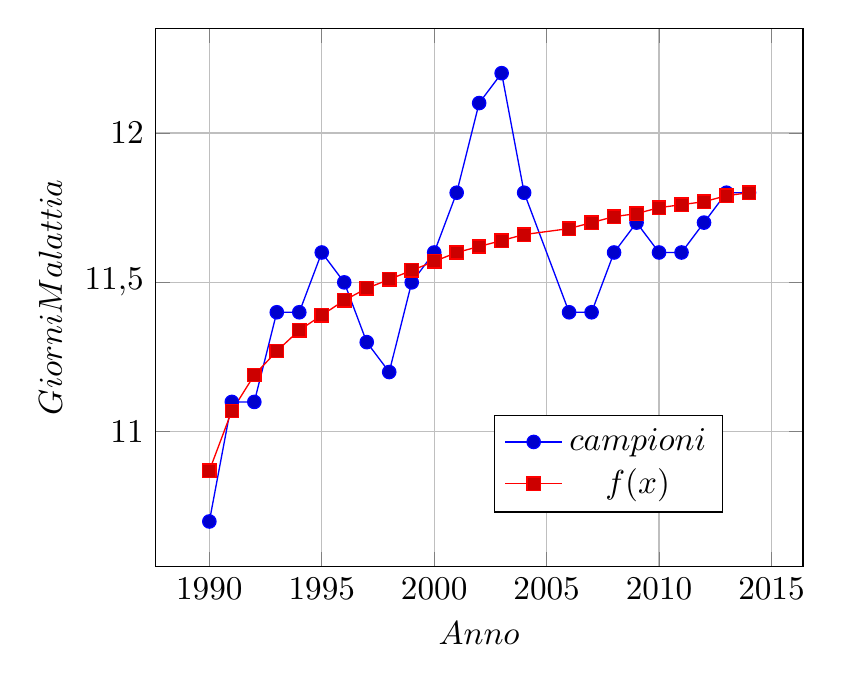
\begin{tikzpicture}[scale=1.2]
 \pgfkeys {
			/pgf/number format/.cd,
			set decimal separator={,{\!}},
			set thousands separator={}}
	\begin{axis}[ xlabel=$Anno$, ylabel=$Giorni Malattia$, grid=major, legend style={anchor=south, at={(0.7,0.1)}} ]
		
		\addplot coordinates{( 1990, 10.7) 
							  ( 1991, 11.1)
							  ( 1992, 11.1)
							  ( 1993, 11.4)
							  ( 1994, 11.4)
							  ( 1995, 11.6)
							  ( 1996, 11.5) 
							  ( 1997, 11.3)
							  ( 1998, 11.2)
							  ( 1999, 11.5)
							  ( 2000, 11.6)
							  ( 2001, 11.8)
							  ( 2002, 12.1)
							  ( 2003, 12.2)
							  ( 2004, 11.8)
							  ( 2006, 11.4)
							  ( 2007, 11.4)
							  ( 2008, 11.6)
							  ( 2009, 11.7)
							  ( 2010, 11.6)
							  ( 2011, 11.6)
							  ( 2012, 11.7)							  
							  ( 2013, 11.8)
							  ( 2014, 11.8)
							  };
							  
		\addplot coordinates{( 1990, 10.87) 
							  ( 1991, 11.07)
							  ( 1992, 11.19)
							  ( 1993, 11.27)
							  ( 1994, 11.34)
							  ( 1995, 11.39)
							  ( 1996, 11.44) 
							  ( 1997, 11.48)
							  ( 1998, 11.51)
							  ( 1999, 11.54)
							  ( 2000, 11.57)
							  ( 2001, 11.60)
							  ( 2002, 11.62)
							  ( 2003, 11.64)
							  ( 2004, 11.66)
							  ( 2006, 11.68)
							  ( 2007, 11.70)
							  ( 2008, 11.72)
							  ( 2009, 11.73)
							  ( 2010, 11.75)
							  ( 2011, 11.76)
							  ( 2012, 11.77)		
							  ( 2013, 11.79)
							  ( 2014, 11.80)
							  };
				\legend{$campioni$,$f(x)$}
	\end{axis}
\end{tikzpicture}